% =====================================================================
%  vessel_figures.tex
%  Figure environments and the elevation table for the two vessel
%  figures produced by fig_vessel.py. Put th_vessel_components.pdf and
%  th_vessel_dimensioned.pdf in images/ on Overleaf.
%
%  Suggested placement: the illustrative figure in the background
%  chapter where the PWR is introduced, the dimensioned figure in the
%  design-basis section of the methodology, next to
%  Table tab:model-geometry, and the table right after it.
%
%  Bib keys used: maruyama_2013 (labgene_primary_sources.bib),
%  ez_aldeen_2025 (references_additions.bib, keep only ONE definition).
% =====================================================================

% ---------------------------------------------------------------------
%  Illustrative figure
% ---------------------------------------------------------------------
\begin{figure}[htbp]
  \centering
  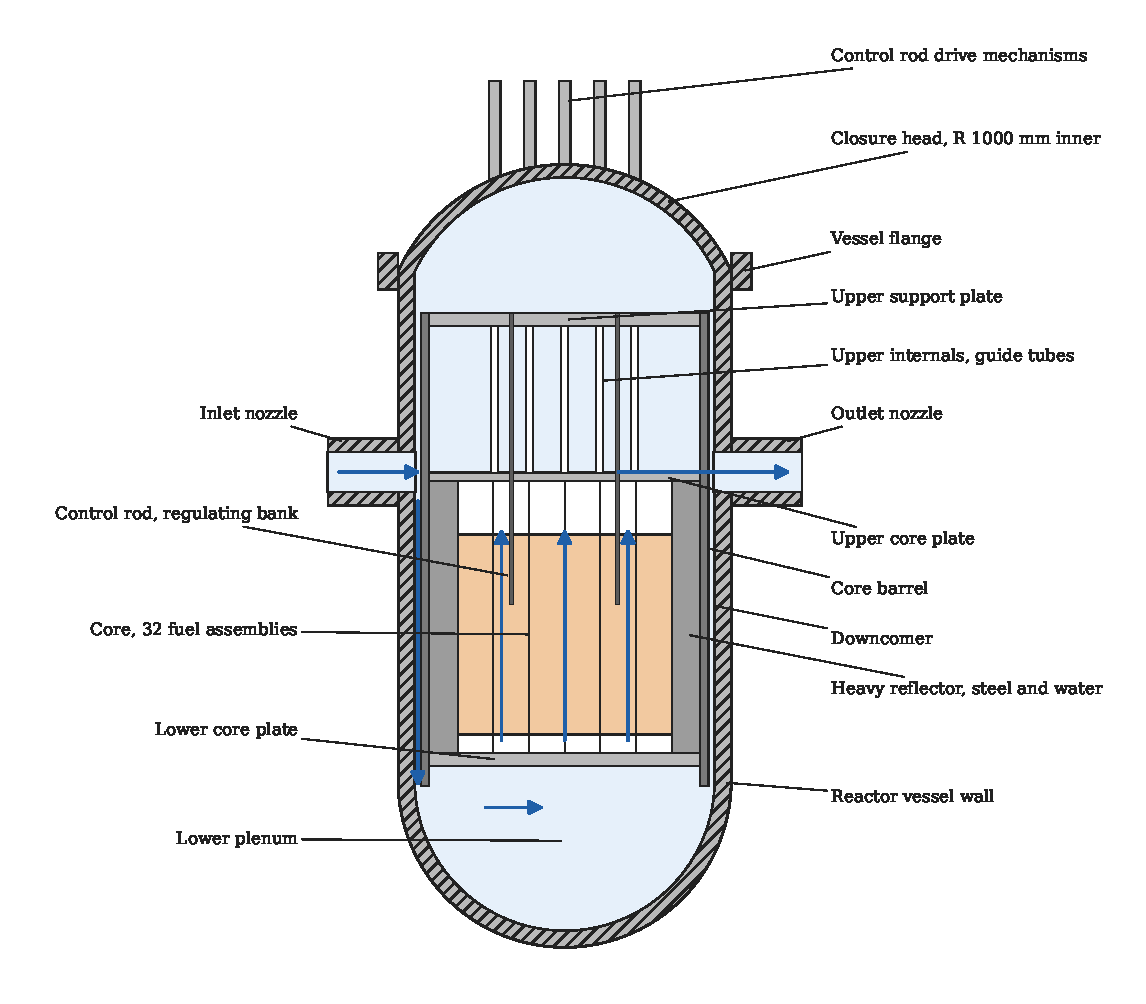
\includegraphics[width=0.95\textwidth]{images/th_vessel_components}
  \caption{Components of a pressurised water reactor vessel, drawn on
    the vessel envelope adopted for the LABGENE-class model. The
    envelope follows the simplified vessel drawing prepared for a
    structural analysis according to CTMSP~\cite{maruyama_2013}. The
    internals, the coolant path and the control rods are illustrative
    and are not to scale. The arrows follow the coolant from the inlet
    nozzle down the downcomer, through the lower plenum and the core,
    to the outlet nozzle.}
  \label{fig:vessel-components}
\end{figure}

% ---------------------------------------------------------------------
%  Dimensioned figure
% ---------------------------------------------------------------------
\begin{figure}[htbp]
  \centering
  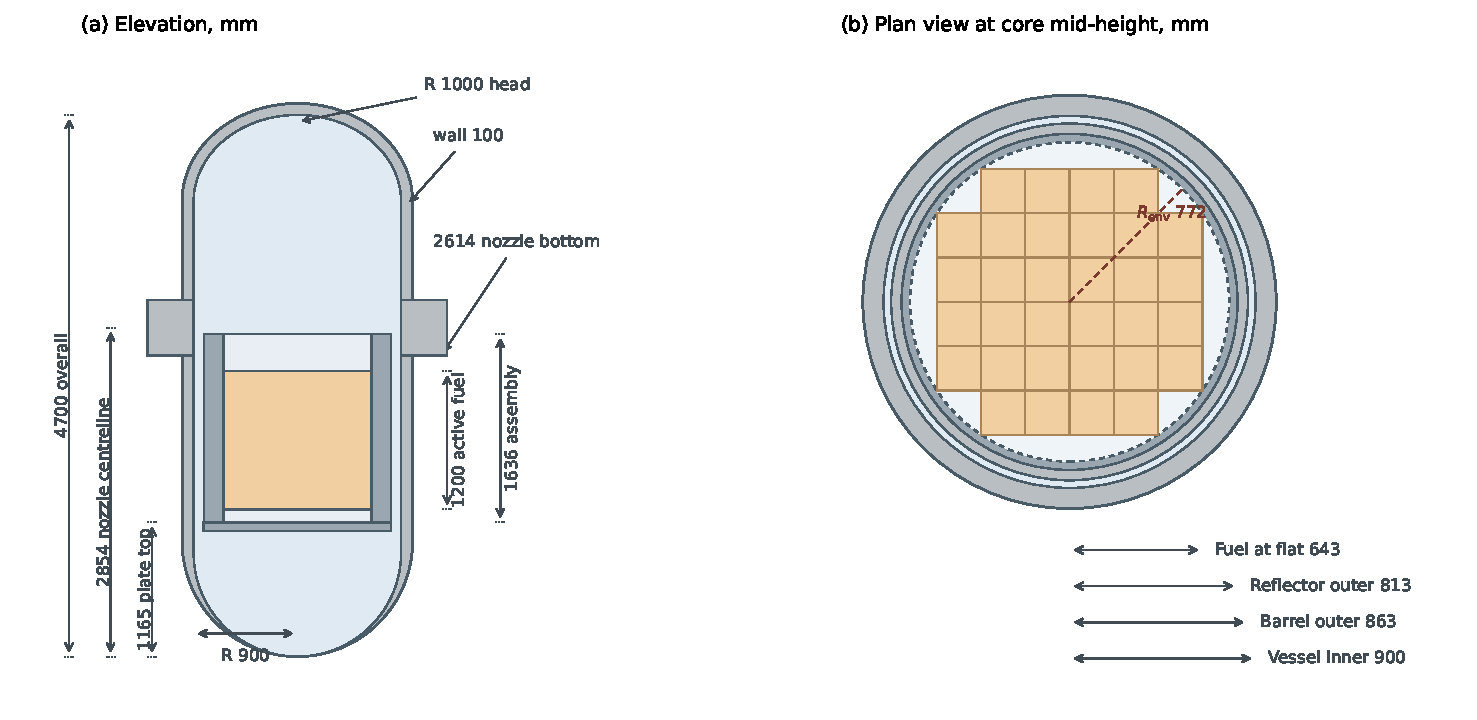
\includegraphics[width=\textwidth]{images/th_vessel_dimensioned}
  \caption{Elevation and plan view of the adopted vessel and core
    layout, in millimetres. The overall height of 4700\,mm, the
    cylindrical inner radius of 900\,mm, the wall thickness of 100\,mm
    and the closure-head inner radius of 1000\,mm are the dimensions
    of the simplified vessel model drawn according to
    CTMSP~\cite{maruyama_2013}. The elevations of the lower core plate
    and of the coolant nozzles were read from the same drawing with the
    4700\,mm dimension as the scale and are estimates. The fuel
    assembly hardware, namely nozzles, end caps, plenum spring and
    spacer grids, is that of the NuScale-like
    benchmark~\cite{ez_aldeen_2025}, kept at the benchmark sizes, with
    the active height of 120\,cm as a modelling choice of this thesis
    and four spacer grids at equal spans. The plan view shows the
    32-assembly footprint, the circumscribed envelope radius
    $R_\mathrm{env}$, the heavy reflector, the core barrel and the
    downcomer for a pin pitch of 1.26\,cm and a minimum reflector
    thickness of 4.0\,cm. The barrel and the downcomer belong to the
    three-dimensional study and are not part of the campaign model.}
  \label{fig:vessel-dimensioned}
\end{figure}

% ---------------------------------------------------------------------
%  Elevation table
% ---------------------------------------------------------------------
\begin{table}[htbp]
  \centering
  \caption{Axial layout adopted for the three-dimensional core model.
    Elevations in millimetres from the outer bottom of the lower head.
    The first two rows are read from~\cite{maruyama_2013}, the hardware
    heights are those of the NuScale-like
    benchmark~\cite{ez_aldeen_2025}, and the active height is the
    design basis of this thesis.}
  \label{tab:axial-layout}
  \begin{tabular}{@{}lrrr@{}}
    \toprule
    \textbf{Item} & \textbf{Height} & \textbf{From} & \textbf{To} \\
    \midrule
    Lower core plate          &   75.0 & 1090.0 & 1165.0 \\
    Coolant nozzle penetration &  481.0 & 2614.0 & 3095.0 \\
    \addlinespace
    Bottom nozzle             &  101.6 & 1165.0 & 1266.6 \\
    Lower end cap             &   12.05 & 1266.6 & 1278.6 \\
    Active fuel               & 1200.0 & 1278.6 & 2478.6 \\
    Plenum spring             &  134.9 & 2478.6 & 2613.5 \\
    Upper end cap             &   12.05 & 2613.5 & 2625.6 \\
    Upper coolant gap         &   84.8 & 2625.6 & 2710.4 \\
    Top nozzle                &   90.2 & 2710.4 & 2800.6 \\
    \addlinespace
    Spacer grid 1, Inconel    &   44.45 & 1314.2 & 1358.6 \\
    Spacer grid 2, Zircaloy   &   44.45 & 1728.3 & 1772.7 \\
    Spacer grid 3, Zircaloy   &   44.45 & 2142.3 & 2186.8 \\
    Spacer grid 4, Zircaloy   &   44.45 & 2556.4 & 2600.8 \\
    \bottomrule
  \end{tabular}
\end{table}

The grid positions follow the benchmark pattern. The first grid starts
35.55\,mm above the fuel bottom, the last grid starts 77.71\,mm above
the fuel top, inside the plenum, and the grids in between sit at equal
spans of 414.1\,mm. The assembly is 1635.6\,mm long, so its top nozzle
ends 187\,mm above the bottom of the coolant nozzle penetration and
53\,mm below the nozzle centreline.
